\section{\large 理論}
\subsection{電気二重層}
\par 水のような誘電率が非常に大きい溶媒にコロイド粒子が分散しているとき,コロイド表面にある解離基からイオンが放出されて粒子表面は電荷を帯びる.放出されたイオンは粒子表面に引き寄せられるが,同時に熱ゆらぎによって拡散され,コロイド粒子周りに電気二重層と呼ばれるイオン雲を形成する.これを定量的に扱う基礎式として,以下に示すPoisson-Boltzmann方程式がある.
\subsubsection{Poisson-Boltzmann方程式}
%
外部電場がないとき,イオンの平衡分布を求める.
化学ポテンシャルが一様になったとき,平衡イオン分布として
\begin{eqnarray}
C^*_{\alpha} = -\sum_\alpha\frac{z_\alpha en_\alpha ^\infty}{\epsilon}\exp(-\frac{z_\alpha e}{k_B T}\psi)
\label{pb}
\end{eqnarray}
\begin{eqnarray}
\nabla\psi ^2 = -\sum_\alpha\frac{z_\alpha en_\alpha ^\infty}{\epsilon}\exp(-\frac{z_\alpha e}{k_B T}\psi)
\label{pb}
\end{eqnarray}
%
ここで,$\psi$は静電ポテンシャル,$z_\alpha$は$\alpha$種のイオン価数である.
%
式(\ref{pb})は偏微分方程式であり,$\psi$が左右の項に現れるため解くことが非常に困難である.
%
$\psi$が十分に小さい場合に次の近似が成り立ち,テイラー展開が可能である.
\begin{eqnarray}
\frac{z_\alpha e}{k_B T}\psi \ll 1
\label{dh}
\end{eqnarray}
%
\begin{eqnarray}
\exp (-\frac{z_\alpha e}{k_B T}\psi)\simeq 1-\frac{z_\alpha e}{k_B T}\psi
\label{taylor}
\end{eqnarray}
%
これを,Debye-H\"uckel近似と言い,以下の式は線形化したPoisson-Boltzmann方程式である.
%
\begin{eqnarray}
\nabla\psi ^2 &=& -\frac{1}{\epsilon}[\sum_\alpha z_\alpha en_\alpha ^\infty - \sum_\alpha\frac{z_\alpha ^2 e^2 n_\alpha ^\infty}{k_B T}\psi]\\
\label{lpb1}
&=&\sum_\alpha\frac{z_\alpha ^2 e^2 n_\alpha ^\infty}{k_B T}\psi\\
\label{lpb2}
&=&\kappa ^2 \psi \\
\label{lpb3}
\kappa ^{-1} &\equiv& (\sum_\alpha\frac{k_B T}{z_\alpha ^2 e^2 n_\alpha ^\infty})
\label{debye l}
\end{eqnarray}
%
式(\ref{lpb1})の右辺第一項$\sum_\alpha z_\alpha en_\alpha ^\infty$は,溶液が電気的に中性のため0となる.
%
ここで出てきた$\kappa ^{-1}$は,電気二重層の厚さの指標となる長さの単位を持つもので,デバイ長さという.
%
球対称な系を考え,$\psi$が$r$だけの関数であるとして式を解くと以下のようになる.
%
\begin{eqnarray}
\psi (r) &=& \frac{eZ'}{4\pi \epsilon}\frac{\exp (-\kappa r)}{r}\\
\label{answer}
Z' &=& \frac{z\exp (\kappa a)}{1+\kappa a}\\
%\label{lpb2}
\end{eqnarray}
%
式(\ref{answer})より,静電ポテンシャル$U(r)$と静電気力$F(r)$が次のように求められる.
%
\begin{eqnarray}
V(r) &=& \int \psi (r)\rho_e (r)dr=\frac{e^2 Z'^2}{4\pi \epsilon}\frac{\exp (-\kappa r)}{r}\\
%\label{answer}
F(r) &=& -\nabla U(r)=\frac{e^2 Z'^2 \kappa ^2}{4\pi \epsilon}\exp (-\kappa r)(\frac{1}{\kappa r}+\frac{1}{(\kappa r)^2})
%\label{lpb2}
\end{eqnarray}
%
これを,$F^* (r)=F(r)\frac{4\pi \epsilon}{e^2 Z'^2 \kappa ^2}$,$r^* =\kappa r$と無次元化すると,
%
\begin{equation}
F^* (r)=\exp (-r^*)(\frac{1}{r^*}+\frac{1}{r^{*2}})
%\label{taylor}
\end{equation}
%
を得る.
\begin{figure}[H]
\centering
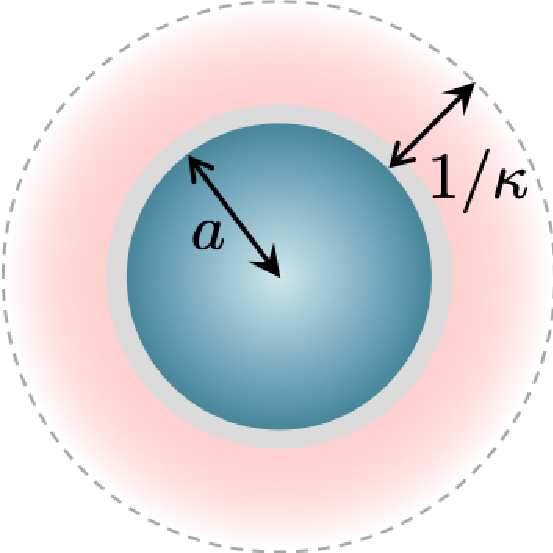
\includegraphics[scale = 0.7]{figures/ka.pdf}
\caption{粒子周りの電気二重層}
\label{ka}
\end{figure}
\noindent
\subsection{電気泳動}
\par 帯電したコロイド粒子に外部から電場をかけると,帯電の度合い・電場の大きさに応じた速度でコロイド粒子が動く.これが電気泳動と呼ばれる現象である.電気泳動のような界面動電現象では,粒子とイオン分布の挙動は流体力学的相互作用と静電相互作用の兼ね合いによって決まる.両者の競合の結果としてイオン分布が球対称から歪み分極することや,イオン雲が粒子から脱げて粒子が裸のまま運動することも起こりうる.本研究で用いたコロイド・微粒子シミュレータKAPSELでは,SPMという手法を用いることにより,コロイド粒子分散系の動的挙動を決定する上で重要な流体力学と静電相互作用を基礎方程式に忠実に数値計算を行っている.
